% Editable source for fig:algorithm. Rebuild with make in this directory.
\documentclass[12pt,border=0pt]{standalone}
\usepackage{times,amsmath,amssymb,tikz}
\usetikzlibrary{intersections,arrows.meta}
\newcommand{\K}{\mathcal K}
\newcommand{\eps}{\varepsilon}

\begin{document}
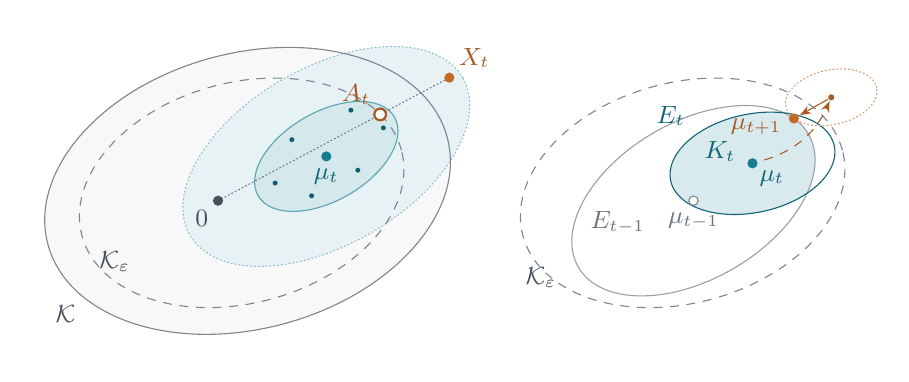
\begin{tikzpicture}[x=1.25cm,y=1.25cm,font=\small,line cap=round,line join=round]
    \definecolor{onsloss}{HTML}{46515B}
    \definecolor{onssmooth}{HTML}{147D92}
    \definecolor{onsquad}{HTML}{C46A29}
    % K is an ellipse containing the origin, and K_eps=(1-eps)K with eps=1/5.
    \tikzset{
        Kshape/.style={rotate around={15:(0.3,0.1)}},
        dot/.style={circle,inner sep=1.3pt,fill=#1},
    }

    %%%%%%%%%%%%%%%% left: sampling and playing %%%%%%%%%%%%%%%%
    \begin{scope}
        \fill[onsloss!4,Kshape] (0.3,0.1) ellipse (2.1 and 1.4);
        \node[onsloss] at (-1.55,-1.15) {$\K$};
        \node[onsloss] at (-1.05,-0.62) {$\K_\eps$};

        % the sampling distribution: two level sets around the mean
        \fill[onssmooth!10,rotate around={30:(1.1,0.45)}] (1.1,0.45) ellipse (1.6 and 0.9);
        \fill[onssmooth!18,rotate around={30:(1.1,0.45)}] (1.1,0.45) ellipse (0.8 and 0.45);
        \draw[onssmooth!70,thin,rotate around={30:(1.1,0.45)}] (1.1,0.45) ellipse (0.8 and 0.45);
        \draw[onssmooth!50,thin,densely dotted,rotate around={30:(1.1,0.45)}] (1.1,0.45) ellipse (1.6 and 0.9);
        \foreach \p in {(0.75,0.62),(1.42,0.31),(0.95,0.05),(1.35,0.92),(0.58,0.18),(1.68,0.74)}
            \fill[onssmooth!75!black] \p circle[radius=0.9pt];
        \draw[onsloss!70,thin,Kshape] (0.3,0.1) ellipse (2.1 and 1.4);
        \draw[onsloss!70,thin,dashed,name path=Keps,scale=0.8,Kshape] (0.3,0.1) ellipse (2.1 and 1.4);
        \node[dot=onssmooth] (mu) at (1.1,0.45) {};
        \node[below=1pt,text=onssmooth!80!black] at (mu) {$\mu_t$};

        % a sample outside K_eps and the point that is played
        \path[name path=ray] (0,0) -- (2.35,1.25);
        \path[name intersections={of=Keps and ray,by=A}];
        \draw[onsloss!80,densely dotted,thin] (0,0) -- (2.35,1.25);
        \node[dot=onsloss] (O) at (0,0) {};
        \node[below left=0pt,text=onsloss] at (O) {$0$};
        \node[dot=onsquad] (X) at (2.35,1.25) {};
        \node[above right=0pt,text=onsquad!85!black] at (X) {$X_t$};
        \node[circle,inner sep=1.5pt,draw=onsquad!85!black,fill=white,line width=0.8pt] (Ad) at (A) {};
        \node[above left=0pt,text=onsquad!85!black] at (A) {$A_t$};
    \end{scope}

    %%%%%%%%%%%%%%%% right: the update %%%%%%%%%%%%%%%%
    % E_{t-1}: centre (0.35,0), semiaxes (1.35,0.8), angle 30.
    % E_t: centre mu_t=(0.95,0.38), semiaxes (0.85,0.5), angle 12.
    % The Newton step ends at (1.75,1.05). Its projection onto K_t in the norm
    % whose unit ball has the shape of E_t is (1.371,0.835), computed numerically;
    % the dotted ellipse is the ball of that norm around (1.75,1.05) that touches K_t.
    \begin{scope}[xshift=5.6cm]
        \draw[onsloss!70,thin,dashed,scale=0.8,Kshape] (0.3,0.1) ellipse (2.1 and 1.4);
        \node[onsloss] at (-1.2,-0.78) {$\K_\eps$};
        \begin{scope}
            \clip[scale=0.8,Kshape] (0.3,0.1) ellipse (2.1 and 1.4);
            \clip[rotate around={30:(0.35,0)}] (0.35,0) ellipse (1.35 and 0.8);
            \fill[onssmooth!16,rotate around={12:(0.95,0.38)}] (0.95,0.38) ellipse (0.85 and 0.5);
        \end{scope}
        \draw[onsloss!55,thin,rotate around={30:(0.35,0)}] (0.35,0) ellipse (1.35 and 0.8);
        \draw[onssmooth!80!black,thin,rotate around={12:(0.95,0.38)}] (0.95,0.38) ellipse (0.85 and 0.5);
        \node[onsloss!80] at (-0.42,-0.22) {$E_{t-1}$};
        \node[onssmooth!80!black] at (0.12,0.86) {$E_t$};
        \node[onssmooth!80!black] at (0.62,0.5) {$K_t$};

        \node[circle,inner sep=1.2pt,draw=onsloss!70,fill=white] (mup) at (0.35,0) {};
        \node[below=1pt,text=onsloss!80] at (mup) {$\mu_{t-1}$};
        \node[dot=onssmooth] (mu) at (0.95,0.38) {};
        \node[below right=-1pt,text=onssmooth!80!black] at (mu) {$\mu_t$};

        \coordinate (c) at (1.75,1.05);
        \coordinate (m) at (1.371,0.835);
        \draw[onsquad!70,thin,densely dotted,rotate around={12:(c)}] (c) ellipse (0.472 and 0.278);
        \draw[onsquad!85!black,thin,dashed,-{Stealth[length=4pt]},shorten <=2.5pt,shorten >=1.5pt] (mu) to[bend right=25] (c);
        \fill[onsquad!85!black] (c) circle[radius=1.1pt];
        \draw[onsquad!85!black,thin,-{Stealth[length=4pt]},shorten <=1.5pt,shorten >=2.5pt] (c) -- (m);
        \node[dot=onsquad] at (m) {};
        \node[left=1pt,yshift=-3pt,text=onsquad!85!black] at (m) {$\mu_{t+1}$};
    \end{scope}
\end{tikzpicture}
\end{document}
